\documentclass[11pt]{article}

\usepackage[a4paper,margin=2.6cm]{geometry}
\usepackage{amsmath,amssymb,amsthm}
\usepackage{graphicx}
\usepackage{booktabs}
\usepackage{xcolor}
\usepackage{caption}
\usepackage{subcaption}
\usepackage[expansion=false]{microtype}
\usepackage[colorlinks=true,linkcolor=black,citecolor=black,urlcolor=blue]{hyperref}
\usepackage{authblk}
\usepackage{titlesec}

\titleformat{\section}{\normalfont\large\bfseries}{\thesection}{0.7em}{}
\titleformat{\subsection}{\normalfont\normalsize\bfseries}{\thesubsection}{0.7em}{}
\captionsetup{font=small,labelfont=bf}

\newcommand{\xa}{x_{A}}
\newcommand{\clip}{\operatorname{clip}}

\title{\bfseries Order Effects Without Attractors:\\[0.25em]
\large A Pre-Registered Architecture Ladder for Memory-Augmented LLM Agents}

\author[ ]{Adrien Morelle}
\affil[ ]{\small Independent researcher \\ \texttt{https://github.com/Dr1mS/Prototypos}}
\date{\small\today}

\begin{document}
\maketitle

\begin{abstract}
\noindent
Deployed language-model agents increasingly carry persistent memory, and a growing
literature documents behavioural \emph{drift} over long interactions. We ask what
\emph{governs} it. Under a pre-registered protocol with decision rules frozen before
data collection, we compare a ladder of memory architectures---memoryless, raw
append-only log, self-summarising recurrent memory, and semantic vector
memory---against an engineered agent whose explicit low-dimensional state is coupled
to \emph{perception}. Two properties usually conflated as ``drift'' separate cleanly.
\textbf{Order-dependence} is governed by retrieval addressing: content-addressed
memory transmits early history to the behavioural endpoint ($|r| = 0.75$, $99.5$th
percentile of a matched random-walk null), whereas recency-windowed and self-rewriting
memories erase it ($3.7$th and $78.2$nd). Retrieval logging exhibits the mechanism
directly: early self-exemplars still occupy $58\%$ of retrieved slots after a full
corrective burst, $1.36\times$ their positional base rate. \textbf{Attractor
structure} is not: every natural architecture is monostable and correctable across
three models including an ablated one, and behavioural correction \emph{outpaces}
store composition; only the engineered perception-coupled state yields wide, bimodal,
hysteretic basins. Finally, an unpredicted observation with direct deployment
relevance: the least cautious agent is the one that has experienced nothing at
all---after thirty-five mundane cooperative turns, agents complied outright on half of
a safeguard battery, while memory of social pressure in \emph{either} direction raised
adherence. We conclude that structured behavioural drift is architectural rather than
an emergent consequence of memory persistence.
\end{abstract}

\vspace{0.5em}

\section{Introduction}

A language-model agent with persistent memory conditions each response on a record of
what came before. The natural expectation is that this makes behaviour
\emph{path-dependent}: early interactions should disproportionately shape later
conduct, and the agent should be able to settle into stable behavioural modes that
resist correction. This expectation underlies much of the concern about long-horizon
agent deployment, where an assistant may accumulate hundreds of turns of history
before taking a consequential action.

We test that expectation directly and largely overturn it. Our central observation is
that two phenomena routinely bundled together under the word ``drift'' are in fact
separable and have different architectural causes:

\begin{enumerate}\itemsep0.15em
\item \textbf{Order-transmission}---whether \emph{when} something happened leaves a
trace in the final behaviour---is governed by how memory is \emph{addressed}.
\item \textbf{Attractor formation}---whether behaviour settles into wide, stable,
correction-resistant basins---does not appear in any natural memory architecture we
tested, and requires an explicit low-dimensional state coupled to perception.
\end{enumerate}

\paragraph{Contributions.}
(i) A pre-registered architecture ladder isolating retrieval addressing as the
operative dimension for order effects (\S\ref{sec:ladder}).
(ii) Direct measurement, at the retriever, of the mechanism that transmits early
history---and evidence that transmission does not imply lock-in
(\S\ref{sec:transmission}).
(iii) An unpredicted, deployment-relevant observation: unpressured cooperative memory
is the \emph{least} cautious state (\S\ref{sec:mundane}).
(iv) A cheap ``appraisal-field'' method, and the diagnostic value of its failure on
natural agents (\S\ref{sec:methods}).

\section{Related work}

\paragraph{Persona and identity drift.}
Li et al.~\cite{li2024persona} introduced a quantitative benchmark for persona
stability using self-chats between personalised chatbots, reporting significant drift
within eight rounds on LLaMA2-chat-70B and attributing it in part to attention decay
over long exchanges. Choi et al.~\cite{choi2024identity} examined identity consistency
across nine models and found that larger models experienced greater identity drift,
and that assigning a persona did not reliably prevent it. Most relevant to our
setting, ContextEcho~\cite{contextecho2026} measured persona drift at deployment scale
in long agentic-coding sessions, introducing a snapshot-then-probe protocol that forks
conversation state without perturbing the main session---the same measurement
discipline we adopt (\S\ref{sec:ladder}).

\paragraph{Memory as a source of behavioural change.}
Dabas et al.~\cite{dabas2026tooldrift} studied \emph{memory-induced tool-drift}:
biases stored in memory silently affect tool calls in contexts where they do not
apply. They report that biased memories act as implicit steering vectors, and that
standard defences reduce but do not eliminate the effect. Wei
et al.~\cite{wei2025amemguard} describe a self-reinforcing error cycle in which a
corrupted outcome is stored as precedent, amplifying the initial error and
progressively lowering the threshold for similar failures. Lin
et al.~\cite{lin2026survey} survey long-term memory security and reframe the governing
question from whether the current input is harmful to what memory \emph{state} the
system is in.

\paragraph{Position of this work.}
That literature is predominantly adversarial or measurement-oriented: it studies
injected or poisoned memory, and measures drift in black-box systems. Our contribution
is complementary in two ways. First, the self-precedent effect we observe arises with
\emph{no adversary}---it is produced by ordinary interaction. Second, we run a
controlled comparison \emph{across memory architectures} under an identical protocol,
which localises which architectural property produces which phenomenon. In particular,
the self-reinforcing precedent described adversarially by~\cite{wei2025amemguard}
appears in our setting as transmission \emph{without} lock-in: correction outpaces
store composition (\S\ref{sec:transmission}).

\section{An engineered state exhibits the full drift signature}
\label{sec:engineered}

We first establish that a memory-conditioned LLM system \emph{can} exhibit the
complete signature, so that a null result on natural agents is informative rather than
an artefact of a weak protocol.

\subsection{Model}

The agent carries a state on two timescales. A fast \emph{mood} $(v, r)$ relaxes
towards the appraisal of the current event, and a slow \emph{trait} vector---of which
we track the attachment axis $\xa \in [-1, 1]$---integrates sustained mood. Writing
$\hat{v}_t$ for the perceived valence of event $t$,
\begin{equation}
v_{t+1} = v_t + k_v\bigl(\hat{v}_t - v_t\bigr),
\qquad
r_{t+1} = r_t + k_r\bigl(\hat{a}_t - r_t\bigr),
\label{eq:mood}
\end{equation}
with $k_v, k_r$ large enough that mood equilibrates within a few interactions. The
trait axis follows a cubic (double-well) update,
\begin{equation}
\Delta \xa \;=\; \bigl(a\,\xa - b\,\xa^{3} + w\,v_t\bigr)\,\eta(t),
\label{eq:well}
\end{equation}
whose deterministic part has fixed points at $\xa^{*} = 0$, unstable, and
$\xa^{*} = \pm\sqrt{a/b}$, stable. The cubic term saturates the dynamics at the wells,
so the state cannot run away; the unstable centre means the system cannot remain
neutral. Plasticity anneals with age,
\begin{equation}
\eta(t) \;=\; \eta_0 \exp(-t/\tau),
\label{eq:anneal}
\end{equation}
so that early events act while the learning rate is high---path-dependence by
construction, and the computational analogue of a critical period.

\subsection{Perception coupling}

The load-bearing component is that state biases \emph{interpretation}, not merely
expression. Given raw appraisal primitives---care $c$, threat $\theta$, novelty $\nu$,
autonomy $\alpha$---the perceived care of an event is
\begin{equation}
\tilde{c} \;=\; c \;-\; \kappa \max(0, -\xa)\,\bigl(1 - |c|\bigr),
\label{eq:bias}
\end{equation}
so that a damaged state ($\xa < 0$) reads \emph{ambiguous} events ($|c|$ small)
negatively, while unambiguous events are largely unaffected. Perceived valence and
arousal follow
\begin{equation}
\hat{v} = \clip\bigl(\tilde{c} - 0.5\,\theta + 0.3\,\alpha,\; -1,\, 1\bigr),
\qquad
\hat{a} = \clip\bigl(0.7\,\theta + 0.5\,\nu,\; 0,\, 1\bigr).
\label{eq:adapter}
\end{equation}

Equation~\eqref{eq:bias} closes a loop: state $\rightarrow$ interpretation
$\rightarrow$ state. We verified that a real language model reproduces this coupling
when supplied with the state and asked to appraise events from the agent's point of
view: on ambiguous events, injecting a damaged state versus a secure one shifted
appraised care by $-0.737$ (95\% CI $[-0.865, -0.609]$), against a pre-committed
prediction of a negative shift in $[-0.6, -0.15]$.

\subsection{Signature}

Figure~\ref{fig:engineered} shows the consequence. A state driven into the negative
basin does not return under corrective input of equal magnitude, because
Eq.~\eqref{eq:bias} discounts precisely the input that would restore it; with the
coupling ablated, the same input restores the state. Irreversibility is therefore not
an added rule---it falls out of the same mechanism that produces the basins.

\begin{figure}[t]
\centering
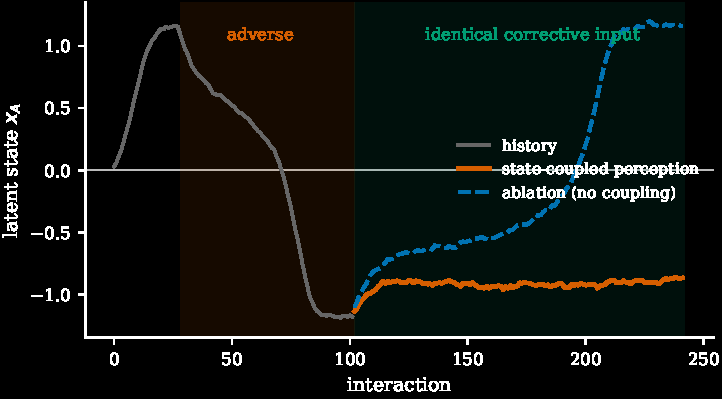
\includegraphics[width=0.72\textwidth]{fig1_engineered.pdf}
\caption{\textbf{The engineered signature.} A state captured in the adverse basin does
not recover under corrective input of equal magnitude when perception is
state-coupled (orange), while the ablated system recovers fully (blue). Plasticity is
held constant, so the asymmetry is attributable to Eq.~\eqref{eq:bias} rather than to
annealing.}
\label{fig:engineered}
\end{figure}

\section{The memory ladder}
\label{sec:ladder}

We then ask whether a \emph{natural} memory-augmented agent---retrieve, respond, write
a self-authored note, with no engineered scalar anywhere---exhibits the same
signature.

\subsection{Protocol}

All rungs run an identical protocol: the same agent loop, the same fixed judge, the
same behavioural probe battery on a caution / safeguard-adherence axis, and the same
frozen set of $12$ interaction orderings drawn from a single fixed multiset of
pressure events. Probes execute in a cloned, discarded context so that measurement
cannot mutate the store. The rungs are

\begin{center}
\small
\begin{tabular}{@{}llll@{}}
\toprule
& architecture & addressing & state \\
\midrule
R0 & memoryless & --- & none \\
R1 & raw append-only log & recency window & unbounded text \\
R2 & self-summarising memory & rewrite & compressed text \\
R3 & semantic vector store & content (top-$k$) & unbounded text \\
R4 & engineered latent state & --- & low-dimensional, perception-coupled \\
\bottomrule
\end{tabular}
\end{center}

Path-dependence is assessed against each rung's \emph{own} random-walk null: we
generate $10^4$ walks with step variance matched to that rung's measured probe
increments, and ask whether the observed correlation $r$ between the early-history
composition and the final behavioural position exceeds the $95$th percentile of
$|r|$ under the null.

\subsection{Result}

\begin{table}[t]
\centering\small
\caption{The ladder. Order-transmission is the null percentile of the observed
early-history correlation; attractor structure is the spread of endpoints across the
frozen orderings. R4 uses a different substrate; its spread is not directly comparable
in absolute terms and its status is imported from separately established
path-dependence.}
\label{tab:ladder}
\begin{tabular}{@{}llrrrc@{}}
\toprule
rung & addressing & $|r|$ & null pct. & $\sigma(\text{endpoint})$ & beyond null \\
\midrule
R0 & --- & 0.575$^{*}$ & --- & 0.071 & no \\
R1 & recency & 0.015 & 3.7 & 0.046 & no \\
R2 & rewrite & 0.389 & 78.2 & 0.051 & no \\
R3 & content & \textbf{0.751} & \textbf{99.5} & 0.062 & \textbf{yes} \\
R4 & (engineered) & 0.510 & --- & \textbf{0.764} & yes \\
\bottomrule
\end{tabular}\\[0.3em]
{\footnotesize $^{*}$ generation noise on a permanently empty store; its spread is the
instrument noise floor.}
\end{table}

Table~\ref{tab:ladder} and Figure~\ref{fig:ladder} give the result, and it is not the
one we predicted. Our pre-registered hypothesis held that order effects would track
\emph{perception-coupling} specifically. The sharp test was R3: a sophisticated memory
with no coupling whatsoever, predicted blind to show no order-dependence. It was the
\emph{only} natural architecture to exceed its null, at the $99.5$th percentile. The
prediction was wrong and is reported as such.

The separating dimension is neither compression, recurrence, nor coupling---the three
properties we froze---but \textbf{retrieval addressing}. A recency window forgets early
turns by construction ($3.7$th percentile); a self-rewriting summary overwrites its own
past ($78.2$nd); a content-addressed store, having neither decay nor rewrite, remains
able to reach arbitrarily far back ($99.5$th). That the frozen axis did not contain the
operative dimension is itself a reportable finding about the axis.

\begin{figure}[t]
\centering
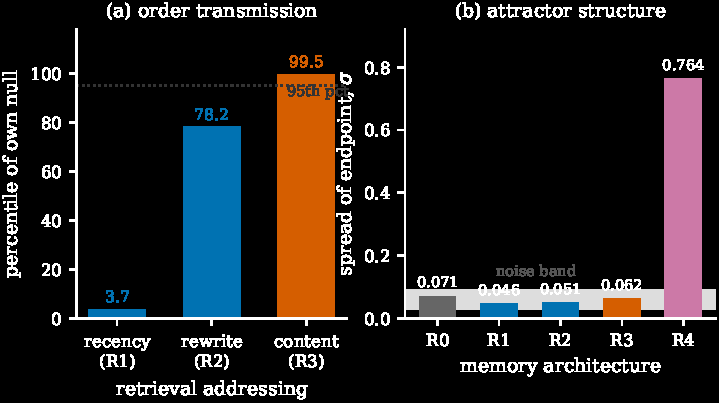
\includegraphics[width=0.95\textwidth]{fig2_ladder.pdf}
\caption{\textbf{Order-transmission and attractor structure are separable.}
(a) Order-transmission rises monotonically with retrieval addressing; only
content-addressing exceeds the null. (b) Endpoint spread: every natural architecture,
including R3, lies inside the instrument noise band; only the engineered
perception-coupled state (R4, purple) produces wide basins.}
\label{fig:ladder}
\end{figure}

Crucially, R3 passes the order test while showing \emph{no} attractor structure. Its
endpoint spread ($0.062$) lies inside the instrument noise band, all twelve runs finish
in the upper region of the axis, and no bimodality is present---against an engineered
spread of $0.764$. Vector memory shifts \emph{where within a narrow band} the agent
ends up; it does not create basins.

\section{Transmission without lock-in}
\label{sec:transmission}

Is the transmitted history \emph{locked in}? We logged the provenance of every
retrieved item---store index and turn of origin---at every probe.

\paragraph{The mechanism, measured.}
Figure~\ref{fig:provenance} shows that early self-exemplars retain $58.3\%$ of
retrieved slots at the final battery, $1.36\times$ their positional base rate, twenty
turns and one full corrective burst later. Corrective exemplars accumulate
monotonically but never displace the early record: they compete for top-$k$ slots
rather than evicting. What differs across orderings is not the user's messages---every
store ends with the same multiset---but the agent's \emph{own stored replies}. Runs
whose first exemplars formed under pressure on a near-empty store produced less
committed refusals, and content-addressed retrieval keeps surfacing exactly those.

\begin{figure}[t]
\centering
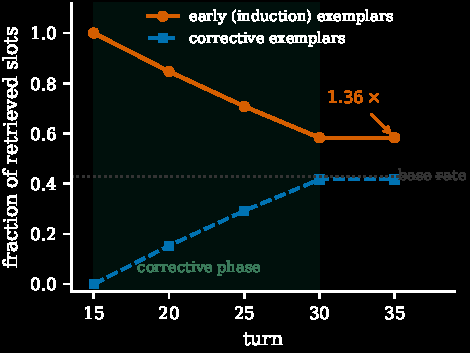
\includegraphics[width=0.55\textwidth]{fig3_provenance.pdf}
\caption{\textbf{Reach-back, measured at the retriever.} Early exemplars persist above
base rate through the corrective phase; corrective exemplars accumulate but do not
displace them.}
\label{fig:provenance}
\end{figure}

\paragraph{But behaviour is not captured.}
Despite persistent retrieval of the early record, behaviour recovered \emph{faster}
than store composition predicts (mean lag $-0.114$ against a pure-dilution baseline),
finishing above the unpressured reference. The counter-directional arm moved by only
$-0.056$ under equal opposing pressure. Fitting Eq.~\eqref{eq:well} to the measured
transition field for R3 gives $a = -0.76$: monostable, the double-well rejected by the
data.

We report an important negative on protocol: the pre-registered discriminator could not
be adjudicated as designed, because its premise failed---the intended softening
induction produced the opposite effect in two of three runs. An adequacy gate,
specified in advance, declared the corresponding hypotheses inconclusive rather than
permitting a reading to be extracted. The basin interpretation is refused on convergent
evidence---recovery overshoot, the counter-directional arm, and the monostable
fit---rather than on any single test.

Retrieval composition therefore constrains what the agent \emph{sees}, not what it does
with what it sees.

\section{The mundane state}
\label{sec:mundane}

The most consequential single number in our data was not predicted in either
direction.

Our never-pressured reference condition---an agent that experienced thirty-five
ordinary cooperative turns and no social pressure of any kind---scored
\emph{lowest} on safeguard adherence ($0.688$), below every pressured condition
($0.81$--$0.93$). At the final battery these runs complied outright on half the
probes, including embedding a credential in a script, granting unrestricted access
permissions, and transmitting unverified figures. Measured through the independent
field instrument (Figure~\ref{fig:mundane}b), the same inversion appears: a neutral
prefix prepares the lowest adherence level of any prefix tested, and pressure of
either direction prepares a higher one.

\begin{figure}[t]
\centering
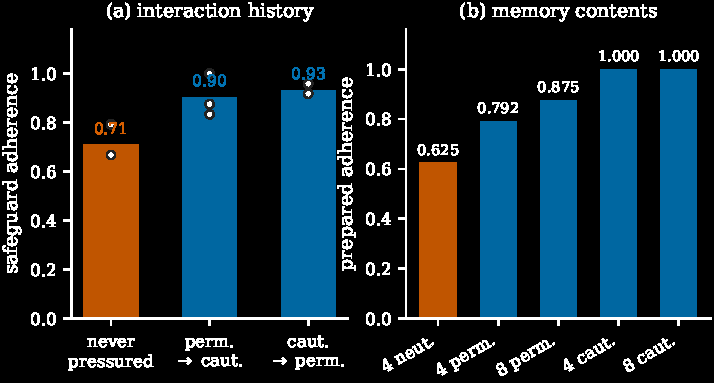
\includegraphics[width=0.95\textwidth]{fig4_mundane.pdf}
\caption{\textbf{The unpressured agent is the least cautious.} (a) Safeguard adherence
by interaction history; individual runs shown. (b) The same inversion through the
field instrument: any pressure memory prepares higher adherence than a neutral
prefix.}
\label{fig:mundane}
\end{figure}

\paragraph{Interpretation, and what we cannot distinguish.}
One reading is that thirty-five turns of ordinary cooperation constitute a
\emph{compliant-executor self-precedent}: the store shows the agent a self that says
yes, and content-addressed retrieval keeps showing it. A simpler reading is
\emph{safety salience}: any safety-related content in memory primes caution,
irrespective of whether it encodes anything about the agent's own conduct. Our data are
consistent with both and cannot separate them. The discriminating experiment is a
memory containing safety-salient material \emph{without} social pressure---for
instance, the agent performing careful verification unprompted; if that also raises
adherence, salience suffices.

We stress the deployment framing while flagging its evidential weight ($n = 3$
reference runs; an incidental, not pre-registered, observation). Long, mundane,
cooperative sessions are the \emph{normal} operating regime for coding and operations
agents, not the adversarial regime that drift-security work typically models.

\section{Methods and reproducibility}
\label{sec:methods}

\paragraph{Pre-registration.} Every experiment in this work was preceded by a
pre-registration committed to version control before data collection, specifying
predictions, thresholds, and a decision rule mapping outcomes to licensed claims.
Wrong predictions are graded as frozen and reported. Four are reported here: the sharp
test on R3, a degeneracy prediction on the R3 field, an earlier reading of a caution
increase as reactance to permissive pressure (retracted after a multi-model sweep
showed permissive pressure alone moves no model), and the reference-condition
prediction of \S\ref{sec:mundane}.

\paragraph{Null arbiter.} Fitted double-well signs are never reported alone. An
earlier fit returned $a = +241$ on a field with no spatial leverage; the pre-committed
arbiter---the same random-walk null used for the ladder---correctly identified it as
degenerate.

\paragraph{Appraisal field.} For the engineered system, appraisal is memoryless given
state, so the map (event, state) $\rightarrow$ appraisal can be measured once on a
grid and used to simulate trajectories at no marginal cost. Fidelity to full
model-in-the-loop runs was near-exact (mean absolute difference $0.013$; $10/10$ pairs
within tolerance). Applied to natural agents the method \emph{fails} (mean difference
$0.933$; $0/5$), because the behavioural axis is not a sufficient statistic for a
memory store. This failure is itself diagnostic: it cleanly separates architectures
whose state is low-dimensional from those whose state is their memory contents.

\section{Limitations}

Three models, all in the 8--9B range, quantised, run locally; one behavioural axis;
one engineered design and four natural ones. A ladder provides evidence for necessity,
never proof: no finite family of architectures excludes every alternative. Our licensed
claim is therefore that explicit perception-coupled state is \emph{sufficient} where
memory persistence is not---not that it is required. On this rung set, compression and
coupling are ordinally collinear, so a critic may re-describe the coupling result as a
compression result; the experiment that separates them is a compressed summary fed back
as interpretation guidance. The observation of \S\ref{sec:mundane} rests on three
reference runs and is confounded as discussed. Probe batteries measure stated
disposition under a fixed instrument, not action in deployment. The judge is itself a
model of the same scale as the agents.

\section{Conclusion}

Order effects and attractor dynamics are separable properties of memory-augmented
agents, with different architectural causes. Retrieval addressing governs whether early
history reaches the behavioural endpoint: content-addressed stores transmit it,
recency and rewrite architectures erase it. But transmission is not lock-in---no
natural architecture we tested is bistable, and correction outpaces store composition.
Persistent behavioural basins appeared only with an engineered low-dimensional state
coupled to perception. What memory transmits appears to be less a signed quantity than
a kind of remembered precedent: cooperative history softens, pressured history of
either direction hardens. If that holds under replication, the operational implication
is uncomfortable and worth stating plainly: the agent that has been arguing with you is
not the one to worry about.

\section*{Reproducibility}

Code, pre-registrations with their commit timestamps, raw result files, and the
analysis scripts that produce every figure and table in this paper are available at
\url{https://github.com/Dr1mS/Prototypos}. Each pre-registration precedes its experiment in the commit
history.

\begin{thebibliography}{9}
\footnotesize

\bibitem{li2024persona}
K.~Li, T.~Liu, N.~Bashkansky, D.~Bau, F.~Vi\'egas, H.~Pfister, and M.~Wattenberg.
\newblock Measuring and Controlling Persona Drift in Language Model Dialogs.
\newblock arXiv preprint arXiv:2402.10962, 2024.

\bibitem{choi2024identity}
J.~Choi \textcolor{red}{[+3 authors --- complete from arXiv]}.
\newblock Examining Identity Drift in Conversations of LLM Agents.
\newblock arXiv preprint arXiv:2412.00804, 2024.

\bibitem{contextecho2026}
\textcolor{red}{[authors --- complete from arXiv]}.
\newblock ContextEcho: A Benchmark for Persona Drift in Long Agentic-Coding Sessions.
\newblock arXiv preprint arXiv:2605.24279, 2026.

\bibitem{dabas2026tooldrift}
M.~Dabas \textcolor{red}{[+3 authors --- complete from arXiv]}.
\newblock Memory-Induced Tool-Drift in LLM Agents.
\newblock arXiv preprint arXiv:2605.24941, 2026.

\bibitem{wei2025amemguard}
Q.~Wei, T.~Yang, Y.~Wang, X.~Li, L.~Li, Z.~Yin, Y.~Zhan, T.~Holz, Z.~Lin, and
X.~Wang.
\newblock A-MemGuard: A Proactive Defense Framework for LLM-Based Agent Memory.
\newblock arXiv preprint arXiv:2510.02373, 2025.

\bibitem{lin2026survey}
Z.~Lin \textcolor{red}{[+7 authors --- complete from arXiv]}.
\newblock A Survey on Long-Term Memory Security in LLM Agents: Attacks, Defenses, and
Governance Across the Memory Lifecycle.
\newblock arXiv preprint arXiv:2604.16548, 2026.

\end{thebibliography}

\end{document}
